%% LaTeX template for BSc Computing for Games final year project dissertations
%% by Edward Powley
%% Games Academy, Falmouth University, UK

%% Based on:
%% bare_jrnl.tex
%% V1.4b
%% 2015/08/26
%% by Michael Shell
%% see http://www.michaelshell.org/
%% for current contact information.
%%
%% This is a skeleton file demonstrating the use of IEEEtran.cls
%% (requires IEEEtran.cls version 1.8b or later) with an IEEE
%% journal paper.
%%
%% Support sites:
%% http://www.michaelshell.org/tex/ieeetran/
%% http://www.ctan.org/pkg/ieeetran
%% and
%% http://www.ieee.org/

%%*************************************************************************
%% Legal Notice:
%% This code is offered as-is without any warranty either expressed or
%% implied; without even the implied warranty of MERCHANTABILITY or
%% FITNESS FOR A PARTICULAR PURPOSE! 
%% User assumes all risk.
%% In no event shall the IEEE or any contributor to this code be liable for
%% any damages or losses, including, but not limited to, incidental,
%% consequential, or any other damages, resulting from the use or misuse
%% of any information contained here.
%%
%% All comments are the opinions of their respective authors and are not
%% necessarily endorsed by the IEEE.
%%
%% This work is distributed under the LaTeX Project Public License (LPPL)
%% ( http://www.latex-project.org/ ) version 1.3, and may be freely used,
%% distributed and modified. A copy of the LPPL, version 1.3, is included
%% in the base LaTeX documentation of all distributions of LaTeX released
%% 2003/12/01 or later.
%% Retain all contribution notices and credits.
%% ** Modified files should be clearly indicated as such, including  **
%% ** renaming them and changing author support contact information. **
%%*************************************************************************


\documentclass[journal]{IEEEtran}

\usepackage{graphicx}
% to embed the file `myreferences.bib` in your `.tex` file
% Insert additional usepackage commands here
\usepackage{color}
\usepackage{listings}
\usepackage[table]{xcolor}
\usepackage{float}
\usepackage{cite}
\usepackage{comment}

\graphicspath{{./Figures/}}

% Select what to do with todonotes: 
%\usepackage[disable]{todonotes} % notes not showed
\usepackage{todonotes}   % notes showed

%%% Remove the next two lines if you want the figures at their place    
%\usepackage[figuresonly,nolists,nomarkers]{endfloat}
%\renewcommand{\processdelayedfloats}{}

\setlength{\arrayrulewidth}{0.5mm}
\setlength{\tabcolsep}{10pt}
%\usepackage{courier} %caused problems for me

%\renewcommand{\includegraphics}[2][]{}
%\renewcommand{\lstinputlisting}[2][]{}

\def\ps@IEEEtitlepagestyle{%
	\def\@oddfoot{\mycopyrightnotice}%
	\def\@evenfoot{}%
}
\def\mycopyrightnotice{%
	{\footnotesize The copyright belongs to me!\hfill}% <--- Change here
	\gdef\mycopyrightnotice{}% just in case
}

\lstloadlanguages{% Check Documentation for further languages ...
	C,
	C++,
	csh,
	Java
}

\definecolor{red}{rgb}{0.6,0,0} % for strings
\definecolor{blue}{rgb}{0,0,0.6}
\definecolor{green}{rgb}{0,0.8,0}
\definecolor{cyan}{rgb}{0.0,0.6,0.6}

\lstset{
	language=csh,
	basicstyle=\footnotesize\ttfamily, 
	numbers=left, 
	numberstyle=\tiny, 
	numbersep=5pt, 
	tabsize=2, 
	extendedchars=true, 
	breaklines=true, 
	frame=b,
	stringstyle=\color{blue}\ttfamily, 
	showspaces=false, 
	showtabs=true, 
	xleftmargin=17pt,
	framexleftmargin=17pt,
	framexrightmargin=5pt,
	framexbottommargin=4pt,
	commentstyle=\color{green},
	morecomment=[l]{//}, %use comment-line-style!
	morecomment=[s]{/*}{*/}, %for multiline comments
	showstringspaces=false, 
	morekeywords={  abstract, event, new, struct,
		as, explicit, null, switch,
		base, extern, object, this,
		bool, false, operator, throw,
		break, finally, out, true,
		byte, fixed, override, try,
		case, float, params, typeof,
		catch, for, private, uint,
		char, foreach, protected, ulong,
		checked, goto, public, unchecked,
		class, if, readonly, unsafe,
		const, implicit, ref, ushort,
		continue, in, return, using,
		decimal, int, sbyte, virtual,
		default, interface, sealed, volatile,
		delegate, internal, short, void,
		do, is, sizeof, while,
		double, lock, stackalloc,
		else, long, static,
		enum, namespace, string},
	keywordstyle=\color{cyan},
	identifierstyle=\color{red},
}
\usepackage{caption}
\DeclareCaptionFont{black}{\color{black}}
\DeclareCaptionFormat{listing}

\begin{document}
	%
	% paper title
	% Titles are generally capitalized except for words such as a, an, and, as,
	% at, but, by, for, in, nor, of, on, or, the, to and up, which are usually
	% not capitalized unless they are the first or last word of the title.
	% Linebreaks \\ can be used within to get better formatting as desired.
	% Do not put math or special symbols in the title.
	\title{%
		To What Degree Can an AI Built With Expert Strategies be Effective Against Competition AI?} %\\
	%\large A Planning Approach to StarCraft AI}
	
	%
	%
	% author name
	\author{\IEEEauthorblockN{James Hellman\\}
		\IEEEauthorblockA{Falmouth Games Academy\\
			UK, Falmouth\\
			Email: jh182233@falmouth.ac.uk\\}
	}
	
	% The paper headers -- please do not change these, but uncomment one of them as appropriate
	% Uncomment this one for COMP320
	%\markboth{COMP320: Research Review and Proposal}{COMP320: Research Review and Proposal}
	% Uncomment this one for COMP360
	\markboth{COMP360: Dissertation}{COMP360: Dissertation}
	
	% make the title area
	\maketitle
	
	% As a general rule, do not put math, special symbols or citations
	% in the abstract or keywords.
	\begin{abstract}
		Effective macro-management (the ability to create armies and expand bases), is essential to obtaining victory in Real-Time Strategy (RTS), in the research community many Artificial Intelligence's (AI's) have been created to handle this. One method is to use a design approach to create what is known as a build order, many of these build orders take from expert strategies used by real people in high ranking tournaments. Build orders can be ridged during games leaving little room for adaptation to the opponent's strategy. In this work, a collection of build orders will be used to create an AI and investigates the impact of build orders that effectively counter strategies used by other Bots. A hypothesis is made here that the AI will only be effective in the early stages of the game and will be outmanoeuvred in late-game stages. Therefore the effectiveness of this AI will be measured its average time survived, with a high average being effective and a low average being ineffective. Whether the AI wins the matches will also be taken into account, a higher average win rate will allow the AI to face a greater challenge. Upon successful completion of this work, the AI will be submitted to one of three competitions.
	\end{abstract}
	
	\section{Introduction}
	\IEEEPARstart{I}{nvestigating} the effectiveness of an AI can be done in many ways, in this work will be looking into the degree of effectiveness an AI built with expert strategies can be against a competitive AI. %First though artificial Intelligence can be defined as anything that gives the illusion of intelligence to an appropriate level \cite{botBook}. 
	In games, AI has been used in both single and multi-player environments to help create a more immersive, challenging and fun experience. One such area which AI is prominent is in the Real-Time Strategy (RTS) genre and since the call for more research to be made for AI in RTS games by Michael Buro in 2004 \cite{CallFor}, research in this area has exploded \cite{Survey}. This has given rise to the creation of many AI's in RTS games, from AI's that are built with pre-defined build orders \cite{Swen} to deep Neural Networks \cite{Deep} that can learn from game-play replays, which will be covered in more detail later on in the paper.
	
	RTS is a great test bed in AI research for its complex systems, involving many areas of interest in planning, dealing with uncertainty, domain knowledge exploitation, task decomposition, spatial reasoning, and machine learning \cite{StarCraftBot}. Unlike turn-based strategy, RTS requires real-time decision making with imperfect information, the information is limited through the use of partial visibility of the map. Unless the AI scouts the map (Sends a unit around the map) and sees what the opponent is doing, then the AI will have no access to any strategic knowledge. This along with the non-deterministic nature of RTS, meaning it may not exhibit the same behaviour on each run, makes RTS one of the most challenging environments in which to create an AI \cite{Current}.
	
	Since the release of StarCraft Brood War API it has been easier for Academics to research AI in StarCraft, this has also given rise to an educational value as part of AI related subjects in several Universities around the world \cite{Current}. One example of this is the University Delft (NL), which for one of its modules the students are required to create a StarCraft Bot \cite{NL}. From this, three yearly competitions have been created to allow students to compete their Bots against other Bots, the first of which was hosted by the University of California, Santa Cruz in 2010 as part of the AAAI Artificial Intelligence and Interactive Digital Entertainment (AIIDE) conference program \cite{AIIDE}. Another hosted at the IEEE Computational Intelligence in Games (CIG) conference \cite{CIG}, and the last one which is an ongoing stand-alone event is the Student StarCraft AI Tournament (SSCAIT) \cite{StarCraftBot}. Upon successful completion of this work, the AI will be submitted to one of these three competitions.
	
	This paper is organised as follows, first StarCraft and what it is will be presented, followed by a review of the current methods being utilized by the research community in the development of StarCraft Bots. With a description on the research that this work will be using, this is proceeded by the method and tools that will be used to create the AI as well the metrics used to measure its effectiveness finishing with the hypothesis. 
	\todo[inline]{Look back to this once conclusion is done to ensure they match}
	
	
	\section{Related Work}
	\subsection{StarCraft}
	StarCraft is an RTS game developed by Blizzard Entertainment \cite{Blizzard} and popular for testing AI \cite{Current}, the game was released in 1998 \cite{Release}. Later that year StarCraft: Brood War was released and took hold in the e-sports community and is still popular today. StarCraft 2: Wings of Liberty was released much later in 2010, with a complete visual overhaul, most of the game mechanics remained the same other than balance changes. The premise of StarCraft is to gather resources, build a base, and build an army to then use to destroy an enemies base and army, during playtime, there are also many upgrades available for these units to give them the edge over an enemy who did not spend the time acquiring them. There are many ways of doing this each player with a different order of building their armies/bases commonly referred to as their "Build Order" \cite{BuildOrder}. Build orders refer to a players macro-management, whereas in StarCraft Micro-management is a huge part of the game, as those with greater control over individual units can better outmanoeuvre their opponent, and thus defeat them. There is a difference in the way units are controlled, in StarCraft:BW you can only select up to 12 units at a time and can not group them for easy selection, so when playing you have to utilise micromanagement skills more than in StarCraft 2 where you can select an unlimited number of units and can group them for easy selection.
	StarCraft is considered difficult due to its requirement of abstraction level thinking when planning. Strategy selection is perhaps the most important choice any player or AI can make in StarCraft and RTS as a whole, as this will dictate the actions and reactions which they take during playtime. Though a human player can be proficient at choosing their strategy by simply scouting the map, finding the enemy and seeing what they are building. The human player can then counter accordingly, and if they countered incorrectly the human player can simply change their strategy to accommodate. Creating an AI to do the same though can be a huge and complex task \cite{Fuzzy,OnlineEvo,GoalDriven}, one way to achieve this result without a large commitment of time is to create a library of expert strategies, and allow the AI to select the appropriate one throughout the game. This can be achieved using tools such as Advanced Behaviour Oriented Design Environment (ABODE) and Parallel-rooted Ordered Slip-stack Hierarchical (POSH) reactive plans \cite{POSH}, which will also be covered later in the paper. These tools allow for an iterative design approach for Bots in games and in this work will be focusing on the macro-management with a particular focus on build orders and the selection of strategies rather than micro-management. 
	
	In this paper, the term Bot which is the standard in the literature will be used rather than AI when referring to AI's that were created specifically for StarCraft. In the StarCraft research community, there are many different methods of Bot creation. Some focus on micro-management like S. Liu et al \cite{EffectiveMicro} that uses a Genetic Algorithm (GA) and others that focus on macro-management looking at the build order like N. Justesen et al \cite{OnlineEvo}. Many of these research methods are cross depended and utilise more than one method, for example, D. Churchill et al \cite{Agents} created the UAlbertaBot, which was intended to automate both build order planning and unit control. There are also Bots that only use one strategy that has won several times in competitions like the ZZZKBot \cite{ZZZK,Results}, which only uses a 3pool build and built that uses a rush tactic. This rush tactic involves creating many weak inexpensive units and sending them to the enemy base within 5 minutes of starting the game. Many Bots tend to struggle with countering this strategy, hence why this type of Bot tends to win.
	
	\subsection{Datasets}
	A Dataset can be a collection of any data, for a game Bot a dataset can consist of thousands of replays with millions of game frames, and player actions\cite{Dataset}. This information can then put together to create a full game-state which allows for machine learning tasks \cite{Dataset17}. In AI research, datasets can be used in many approaches to development, one such use is to recreate game-states and evaluate them for prediction in realistic conditions \cite{SpecialTactics}.
	
	\subsection{Micro-Management}
	Micromanagement is a fundamental side of StarCraft game-play and many papers have their own approach to this aspect of RTS \cite{SOMA,EffectiveMicro,Swarm,MM,SpecialTactics,UnitsControl}. Micromanagement is the control of each unit individually, for example: if you have 12 units, each with their own ability, during battle you need to activate each ability at the correct time for each of the 12 units in order to utilise them to their full potential. This required you to select each unit during battle and activating the ability, while still maintaining control over the other 11 units. Though this is a slight exaggeration as in StarCraft some units have an auto use of their ability which allows the unit to decide when to use their ability, one such unit being the medic on the Terran faction which will heal any biological unit with less than full health. Also in StarCraft units can be selected by type i.e. you can double-click on a marine, and it will select all the marines on screen (Up to a maximum of 12). Players that perfect multitasking micromanagement skills are most likely to win the battles when playing, as they can outmanoeuvre their opponent much more easily and use abilities effectively to devastate the armies of their opponent. Many of these approaches tend to use either Genetic Algorithms (GA) or Evolutionary Algorithms (EA) \cite{SOMA, EffectiveMicro, Swarm}, while others observe replays and apply a Monte-Carlo method to create data for practice use \cite{MM}. But most of these methods have one thing in common, they all use a version of machine learning \cite{Survey}.
	
	\subsection{Predictive Methods}
	On a higher strategic level, the prediction of the opponent's strategy is a prominent approach used in research \cite{DataMine, Bayesian, Scouting, ReplayPred}. This type of research relies on the use of replays and machine learning to help the Bot accurately predict a strategy, these do rely on the quantity and quality of replays used for the learning process\cite{DataMine,Bayesian,ReplayPred}. Another method for prediction is scouting alongside machine learning, this eliminates the need for replay observation and allows for a more real-time prediction \cite{Scouting}. Though this method does still require several games to be played before the Bot can begin to have an accurate prediction.
	
	Bayesian approaches are based on Bayes' Theorem which is another prediction method. Bayes' Theorem is a calculation of probability or also known as a probabilistic model \cite{BayesianAI}. In papers by G. Synnaeve et al \cite{UnitsControl,SpecialTactics} they create a Bot that controls units individually, they do this by using uncertainty which instead of asking where a unit might be, it makes rough estimations and acts upon that. Another use for the Bayesian approach is to predict strategies, by creating a probabilistic model that after learning from replays can predict an opponent's strategy and adapt accordingly \cite{Bayesian}. A major downfall of Bayesian Approaches is that it can be computationally intense to calculate.
	
	\subsection{Full Game Play}
	Many papers try to create a Bot capable of handling all aspects of an RTS \cite{Agents,Hierarchical,HumanLevel,SCAIL}. These Bots tend to take several methods that have been created in other research and combining them to form a new Bot \cite{Agents}. Another use for the full gameplay Bot is to try and create a "Human-Like" Bot, which can mimic the play-style of an expert human player. Though the current Bots are limited in this as players reported that the Bots used unusual unit movements or building placement \cite{EvalHuman}.
	
	\subsection{Neural Networks}
	Neural Networking are computational models loosely based on the functioning of biological brains \cite{Deep}. Given an input it computes an output by using a large number of neural units, in StarCraft it can be used to predict strategies or in the case of StarCraft 2 with its new architecture it can be used for full game-play. Using a neural network would be impractical for the purpose of this work as it would take many months to train, and even then would not have a great chance of doing well against other Bots.
	
	\subsection{Planning}
	Planning in StarCraft usually deals with the build order that the Bot will use usually only dealing with macro-management. There are several different ways to use a build order, some will use a static build order that will not change throughout the game \cite{Swen}, and the more popular route is to allow the Bot to jump between build orders during play-time, another term is Reactive Planning \cite{Fuzzy,OnlineEvo,GoalDriven}. there has been some work on creating the build orders on the fly by finding out that most optimal method of gathering resource and building units \cite{BuildOrder}. Planning is perhaps the most optimal approach to creating a Bot as there are little real-time calculations to make. Through the use of POSH tools \cite{POSH}, you can iteratively design Bot prototypes and deploy quickly \cite{Swen}. 
	
	From looking at the research in the field there are many methods that can be used to create a Bot. The use of replays to train a Bot to counter strategies can be effective \cite{Bayesian}, they lack the greater control of the game, the ability to macro-management as there are too many variables to consider. This lack of large-scale control is usually due to the heavy computational requirements of controlling each individual component of the game.  Due to this slow process, it is quite impractical to use when there is already a library of knowledge that can be to exploited \cite{Liquid}. Though there are Bots out there with planned strategies already programmed into them \cite{ZZZK,Fuzzy}, their limitation is that they only use a small number of strategies, though these work it can leave a lot of room for the opponent to manoeuvre. A logical step here is to program a larger pool of expert knowledge into the Bot, it will then select one and follow it through, with the ability to jump between strategies at key points in-case a counter is detected. 
	
	\subsection{StarCraft Bots}
	In the StarCraft Bot community there are many Bots that have been created to compete against each other, and in this work, a competition Bot is defined as a Bot that has been entered to the Artificial Intelligence for Interactive Digital Entertainment (AIIDE) conference StarCraft Bot Competition. A yearly competition hosted by David Churchill and sponsored by AIIDE. Examples of the top Bots from the competition include:
	\begin{itemize}
		\item ZZZKBot Winner of the 2017 AIIDE StarCraft AI Competition \cite{ZZZK} 
		\item Iron Winner of the 2016 AIIDE StarCraft AI Competition \cite{Iron}
		\item UAlbertaBot Winner of the 2013/2011 AIIDE StarCraft AI Competition \cite{UAlberta}
		\item Skynet Winner of the 2012 AIIDE StarCraft AI Competition \cite{Skynet}
	\end{itemize}
	
	Each of these Bots employ different strategies, these strategies a
	\todo[inline]{Discuss the other Bots and their strategies}
	
	\subsection{Research Questions and Hypothesis}
	
	\subsubsection{Hypothesis}
	\begin{itemize}
		\item \textbf{Hypothesis 1} The Bot will survive no more than 14 minutes and Win.
		\item \textbf{Hypothesis 2} The Bot will have a Win rate greater than 0\%.
		\item \textbf{Hypothesis 3} The Bot will have a Win rate of 50\% or greater.    
		\item \textbf{Hypothesis 4} The Bot will successfully counter the Rush tactic surviving past the 10-minute mark.
	\end{itemize}
	
	\subsubsection{Research Questions}
	During the initial research into this area for this paper other research questions were reviewed:
	\begin{itemize}
		\item Combining Behaviour Oriented Design and Expert Human Knowledge to create a competitive AI.
		
		\item Creating an adaptive AI using predefined expert strategies. 
		
		\item Is an adaptive AI built with predefined expert strategies a viable competitor against non-adaptive AI’s?
		
		\item How effective can an adaptive AI built with predefined expert strategies be against other AI’s?    
	\end{itemize}
	These questions were rejected as creating an adaptive AI was not the focus of this research.
	\newline
	
	\section{Method}
	To answer the question that this paper focuses on, this research will be performing an experiment to gather the empirical data required then performing a positivist analysis on that data, interpreting it through reason and logic, then forming a discussion to defend or reject the hypothesis presented.
	
	\subsection{Tools}
	The tools that will be used in this experiment are; The Brood War Application Programming Interface (BWAPI), POSH tools, specifically POSH Sharp which is an interface that uses c\# instead of C++, and the ABODE editing software which uses POSH plans to create Behaviour Oriented Designs for Bots. Other tools include Visual Studio 2010, Chaoslauncher, StarCraft Tournament Manager, and VirtualBox, all of which will be explained next. 
	
	
	\begin{figure}[H]
		\centering
		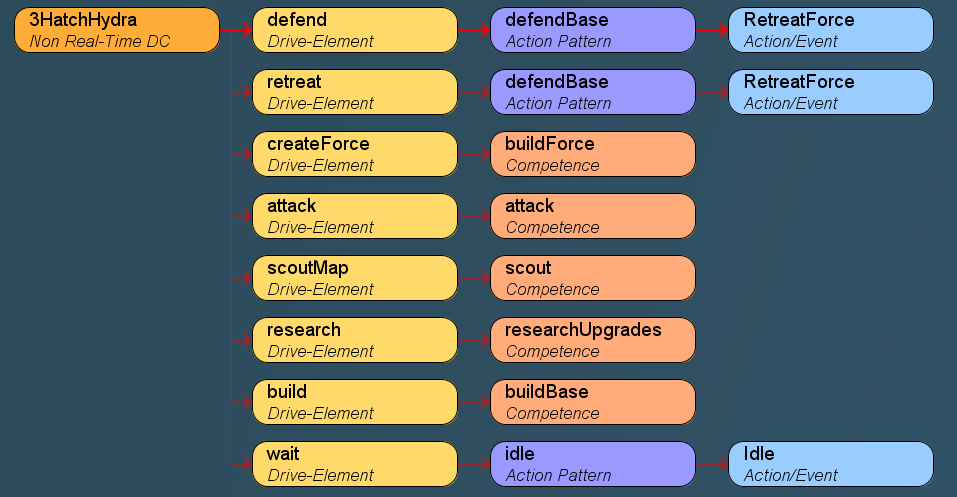
\includegraphics[width=0.5\textwidth]{POSH}
		\caption{POSH plan for the Three Hatch Hydra build plan inside the ABODE editor.}
		\label{Fig1}
	\end{figure}
	
	\begin{itemize}
		\item \textbf{Brood War Application Programming Interface} \cite{BWAPI} is an open source software that creates an interface to allow a custom Bots to communicate with the game. BWAPI only give limited information to the Bot, which inhibits the Bots to have the ability to know what its opponent is doing, this means that the fog of war(the unexplored parts of the map) are is kept\cite{POSH}, this mean that the Bot is just a limited in its knowledge as a player would be. The information that is provided is the size of the map and base locations, this allows the Bot to have the ability to scout effectively. This limited information prevents custom Bots from cheating and ensures a fair game, though for the developers of the Bot this could be considered an advantage for the development stage of the Bot as there is no need to be concerned with accidentally allowing their Bot to access illegal information. This does however provide a challenge in design as the Bot is dealing with imperfect information, it must be designed in such a way that it almost replicated human responses, i.e. scouting, and checking areas already scouted for enemy presence.
		\item[]
		\item \textbf{POSH} plans can be created in the ABODE Environment as seen in Figure 1, these are visual planning tools that allow for a hierarchy of actions with associated triggers. Each plan can be split into three parts, Drive-Collections, Competencies and Action patterns, these three determine when an action is to be triggered. POSH plans use a behaviour library created in the native language of the problem space, see Fig 4. This tool can be a powerful asset to designing and creating an Bot as once the behaviours and senses are implemented new Bot can be created quickly and with little error.
		\item[]
		\item \textbf{Microsoft Visual Studios 2010(VS2010)} is an integrated development environment(SDK) from Microsoft \cite{Visual}. It is used to create computer programs, as well as websites, apps, and online services. In this experiment VS2010 is being used to create the behaviours for the Bot, as well as any other functionality the Bot requires, this includes the framework for the POSH wrapper.
		\item[]
		\item \textbf{Chaoslauncher} is an open source third-party launcher for StarCraft that allows the user to inject any universal plugins \cite{Chaos}. For this experiment, the launcher will be used as a debugging tool for the first stages of the Bot. The launcher also allows StarCraft to be run in windowed mode alongside a BWAPI injector that allows the Bot to communicate with BWAPI.    
		\item[]
		\item \textbf{StarCraft AI Tournament Manager(STM)} is a tool that was developed by David Churchill to manage and run StarCraft AI tournaments, it is an open source project available for anyone to use. It runs the tournament by creating a server and allowing instances of its counterpart (the Client) to connect to it, each client runs a single instance of StarCraft and the server will put two clients into a game and record the results. This set-up allows for as many instances of StarCraft to be run on the server as the user wants, the current set-up of the STM doesn't allow for more than one instance of StarCraft to be run on a single PC at a time. To solve this a Virtual Machine (VM) will be utilized \cite{Tournament}. For the purposes of this experiment the STM will be used to test the Bot against the competition Bots, once the tournament is over the STM will compile a results table similar to fig 2, in an HTML format which can be opened in any browser.
		\begin{figure}
			\centering
			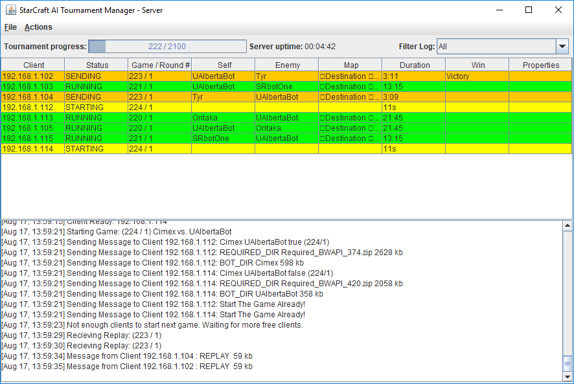
\includegraphics[width=0.5\textwidth]{TMPic}
			\caption{StarCraft Tournament Manager Server Running.}
			\label{Fig2}
		\end{figure}
		\item[]
		\item \textbf{Oracle VirtualBox} is a general-purpose full virtualizer for x86 hardware, targeted at server, desktop and embedded use \cite{Virtual}. This allows the user to run multiple instances of an operating system on the same hardware, for this experiment it will be used to run multiple instances of StarCraft on the same PC. 
		\item[]
		\item \textbf{R} is a language environment for statistical computing, using R along with R studio the user can compute statistical equations and produce the appropriate graphs. For the purposes of this research, R will be used to create some of the figures present in this paper, a code excerpt of R can be seen in fig 3. 
		\newline
	\end{itemize}
	
	\begin{figure}
		\begin{lstlisting}
		[ExecutableAction("SelectProbeScout")]
		public bool SelectProbeScout()
		{
		if (probeScout != null && probeScout.getHitPoints() > 0)
		return true;
		
		Unit scout = null;
		IEnumerable<Unit> units = Interface().GetProbes().Where(probe =>
		probe.getHitPoints() > 0 && !Interface().IsBuilder(probe));
		
		foreach (Unit unit in units)
		{
		if (!unit.isCarryingGas())
		{
		scout = unit;
		break;
		}
		}
		
		if (scout == null && units.Count() > 0)
		{
		scout = units.Last();
		}
		probeScout = scout;
		return (probeScout is Unit && probeScout.getHitPoints() > 0) ? true : false;
		}
		\end{lstlisting}
		\caption{C\# executable action for selecting a probe scout, the plan will execute this code when triggered.}
		\label{Fi4}
	\end{figure}
	
	\subsection{Design and Research Artefact}
	Designing this experiment was a simple, yet time-consuming task once the research question was settled on, the only large design task required was to obtain several expert strategies. These strategies were obtained from an online source Liquipidiea, this is an online wiki available to the esports community to bring together all the information they can to help each other in their respective sports. This wiki is a valuable source of knowledge when trying to obtain the necessary StarCraft strategies as the ones on this site are used by the experts that play the game. 
	
	The challenge was the implementation of these build orders, as the POSH plans have to be precise, meaning the priorities of its actions had to be correct, plus the timing of each action needed to be correct. 
	
	This work will be focusing on the implementation of a Bot with pre-built build orders and their counters taken from Liquipedia \cite{Liquid}, a website dedicated to StarCraft, on the there they have a collection of strategies that are free to use in any capacity. Implementing these build orders are covered in greater detail in Iteration 5: Implementation of New Strategies.
	
	\begin{figure}[H]
		\begin{lstlisting}
		qplot(input$`Win%`, input$Duration, geom = c("point",
		"smooth"), method="rlm", main="Correlation between Win % and Game Duration", xlab="Win %", ylab="Game Duration")
		\end{lstlisting}
		\caption{R code to create a scatter plot with a line of best fit. The figure created from this exert can be seen in Figure 9.}
		\label{Fig3}
	\end{figure}
	
	For the creation of the artefact, there were many options for life cycles that could have been adopted. Chief among these were the incremental model and Agile, both supported short development cycles, but lacked the ability to revisit and refactor code \cite{Life}. For the incremental model, each development cycle is static and isolated, meaning that when the cycle is over the build will never be revisited again. This approach would be an impractical for this artefact as the strategies and variables in the code need to be constantly refactored and tweaked.
	
	The Agile development cycle seemed like a better choice as it is more friendly towards an iterative development cycle that produces smaller chunks of code. Though Agile still lacked the focus on testing first, this was required for this artefact as with each implementation it needed testing to confirm if the implementation succeeded. For this artefact, Agile will be combined with Test Driven Development (TDD) as there is no use of daily scrums, plus the focus of this research is to have a working Bot, and the best method to achieve this is to continuously test and refactor. This method is called Agile Model Driven Development (AMDD) which focuses on iterative development while also being test driven, a more detailed description of this can be found in the appendix under table 7. Another reason for AMDD is that the constant small changes to the code would dramatically affect the functionality of the Bot, therefore every change needs testing.
	
	For testing the only concern was whether a function within the code did as was designed, there is only a pass/fail did it do the thing it was designed for or not, when testing these only one test is usually required to get the answer then a slight modification was made each time if it resulted in a fail. The tests had only minor automation as the artefact had to be manually run and the game manually set-up.
	\newline
	
	\subsubsection{Iteration 0 : Software Installation And Design}
	Before any development was carried out, the first decision was how was the Bot to be created, it could either be done in C++ pure, Java or C\# using POSH-tools. PODH tools were chosen as
	
	The first sprint was to set up the environment. This involved downloading and installing several versions of Visual Studio and downloading the correct version of BWAPI, Chaoslauncher, and the addition of PoshSharp. An intimidate issue that came up after attempting to compile BWAPI, there were missing .ddl's in the Windows directory, to rectify this the relevant dll's were manually copied into the relevant locations. Once the coding environment was set up, the next step before any code was written was to set up the testing environment. This was done using the Chaoslauncher, which would inject BWAPI into the game to allow the Bot to work correctly within the game. Once StarCraft launched with no issues, a basic POSH plan with no functionality, that came with POSHSharp was compiled and executed, this all had to be done in admin mode as it would not work correctly. By the end of this sprint, the correct software was installed, the testing environment was working, and a basic plan ran in the game. The artefact at this point was ready to be designed and have code written in the behaviours.
	
	In this work Protoss will be chosen, this choice was made as Zerg have been done many times and usually rely on rushes to win, whereas Terran are too complex for the planned Bot. Protoss proved a happy middle ground to build upon where rushes are difficult to achieve but they are not too complex that it is too difficult to execute a sound strategy. So the second logical step is to implement an anti-rush strategy as an opening strategy. From there more aggressive strategies will be implemented and executed at the appropriate times. The challenge here is that it is difficult for Protoss to counter a Zerg rush but if successful it will leave the Zerg open for attack. To support this decision the ratio that the races won were looked into and can be seen in fig 4, here the Protoss clearly loose more often than the other two races.
	
	Before any design could commence a race had to be chosen, in StarCraft, there are three, Zerg, Protoss and Terran, each with their own unique play style. Zerg is a rushing faction, with their units being relatively weak and cheap, the Zerg usually focus on overwhelming their enemy with numbers. Protoss are strong but expensive, relying on smaller numbers and taking longer to produce anything, this means they can be weak at rushing and defending from a rush. Terran is a balance of the two, being able to produce strong and expensive units as well as cheap, weak ones, they can effectively rush and defend from a rush.
	
	A rush is a tactic employed in RTS games which involves building up a small force as quickly as possible to harass the enemy base and units. A rush is only considered a rush if it is done within the first five minutes of the game \cite{Liqui}.
	
	Once the software was installed, the method of development was chosen and Protoss was picked, the next step was to begin testing and developing. 
	\newline
	
	\subsubsection{Iteration 1 : Prototype}
	The artefact needed to have an executable plan for the desired race, in this case, Protoss, the reasoning for this is explained in the Method section, under Preliminary Results. No behaviours were changed, this was simply an exercise to ensure the testing environment ran with the correct race, so only basic functionality was present. This functionality would make Probes gather resources and build a Pylon. This would be the final step in setting up the tests, as now the Protoss ran with no issues in game and testing would be seamless.
	\newline
	
	\subsubsection{Iteration 2 : Alpha}
	Creating an alpha involved changing the behaviours to suit the race and the behaviours that came with the software were written for Zerg only. Which meant that there had to be a lot of redesigns and code refactoring needed. An example of this would be the positioning of buildings, for Zerg they can only build on something called "Creep" this is present at the start of the game at a set radius around the starting base and can be extended through the use of special structures. For Protoss however they can only build within range of a structure called a "Pylon", these Pylons can be built anywhere but any other structure bar the starting structure has to be built within range. The behaviour for the placement of structures for Zerg worked fine for them however for the Protoss the function had to be refined for more precision when building. 
	
	Another example is when building structures the Zerg lose a builder, as the builder "Morphs" into the structure so each time something is built the Bot would just select a new builder and remove the previous one from any list it was related to. Protoss, on the other hand, can have many structures constructing at one time, this means that the build must remain the same unit. Plus the Training of units, as Zerg only trained from one structure whereas Protoss would train from several.
	
	This was done over several weeks, every behaviour, action and sense that was modified/written was tested for functionality each and every time there was a change. This allowed the artefact to take small steps with each change and test always progressing. Once a piece of code was complete there was rarely a need to return to it, and if there was then it was a simple matter to make a change and test if it worked. By the end of the sprint, the Bot was building in the correct places and produced units from another structure.
	\newline
	
	\subsubsection{Iteration 3 : Beta}
	During this sprint, the objective was to ensure the Bot could build in other locations as well as build an army to attack the enemy. The first goal was to create a method for the Bot to find the choke point and set it as a base location for building its structures, this also opened up an issue with ensuring the Bot can swap building locations. Within BWAPI the Bot has knowledge of all the choke points and base locations, though they are not allowed to access them unless it has been revealed on the map. then once it has the Bot can save that location, and once it needs to build there it will use the positioning code from that location instead of from the start base. 
	
	Once the functionality for building at the choke was implemented and tested, a plan with greater detail was created. Meaning that the Bot would now take advantage of building at both the starting area as well as the natural expansion and choke point. Along with this the Bot had to build an army and attack the enemy, using the new method for finding new build locations, it was a simple modification to the scouting function to allow the Bot to find the enemy base and mark its location, which allowed the Bot to know where to go with its forces.
	\newline
	
	\subsubsection{Iteration 4 : Polish}
	At the end of this sprint, the Bot was expected to have all behaviours fully implemented and tested and a completed plan written and tested. This was an opportunity to look back and refactor any code that needed tuning or any duplicate code that got into the system. Though the point of TDD is to avoid duplicate code, its priority is to get code that works, in the case of this software duplicate code did end up in the system. Due to the nature of the "Action", "Sense" system there was bound to be duplicate code, though it can be minimized with internal functions.
	\begin{table*}[]
		\centering
		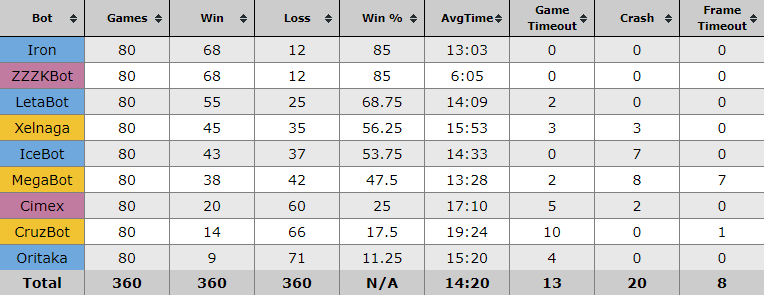
\includegraphics[width=\textwidth]{STMResults}
		\caption{The HTML results table produced by the StarCraft Tournament Manager \cite{Tournament}. Blue represents Terran, Purple represents Zerg, and Yellow represents Protoss}
		\label{Table1}
	\end{table*}
	Tuning the plan took most of the time in this sprint as with each change the plan had to be tested within the game, to ensure that the change was meaningful and effective. This usually involved changing the build order and priority order of actions.
	\newline
	
	\subsubsection{Iteration 5 : Implementation of New Strategies}
	The final sprint was to implement several plans that could work alongside the base plan, these would all be taken from the Liquipidiea site. The current set-up only allows for one plan to be used at a time, though each plan can contain several strategies that are triggered when the Bot plays. Each strategy was tailored to face each race as an opponent, three strategies were chosen from Liquipedia, one for Protoss VS Terran, VS Zerg, and VS Protoss, When two races are the same it is referred to as a mirror match.
	
	Each strategy focuses on the same goal, producing a unit called Dark Templars (DT) as quickly as possible. This Unit is cloaked and has a clear advantage over an enemy that has no detectors (detectors are a unit that can reveal cloaked/hidden units). The process to achieve this can be seen in figure 11 in the Appendix, which shows the tech tree for the Protoss.
	Though each strategy gets to this goal in different ways:
	
	\begin{itemize}
		\item For Protoss VS Zerg the Bot will use a strategy known as "One Base Speedzeal (vz. Zerg)" \cite{PVZ}, the focus is to produce Zealots and as soon as possible produce DT's, once the DT's are in production the Zealots are to move to the Zerg base and harass them until the DT's arrive. At which point the Zerg should either be crippled or defeated, though smart building placement by the Zerg can counter this, then to counter the counter, the Protoss must recover as quickly as possible and renew the attack, or at least continue harassing the Zerg until the Protoss has a large enough army to win.
		\item[]
		\item When facing Terran the Bot will use a strategy known as "2 Gate Dark Templar (vz. Terran)" \cite{PVT}, the Bot must forego the Zealots and head straight into DT's, the means that the Protoss are prone to early rushes by the enemy, but to defend against this one or two ranges units called Dragoons are trained to defend. Once the Protoss has two DT's they are sent to the enemies natural expansion to harass them and lock them in their base unit the Protoss are ready to finish them off.
		\item[]
		\item The hardest strategy to implement is for the mirror Protoss VS Protoss, as they both can produce the same units at the same rate. The Bot will use a strategy known as "2 Gateway Dark Templar (vz. Protoss) \cite{PVP}, DT's are again used in this instance. Though this strategy employs tactics from both other strategies, building Zealots and Dragoons for both attack and defence. Photon cannons (A defensive structure) are used to help defend against any attacks. Once the initial attack was defended, and the natural expansion taken the focus shifts to mass producing units, and sending them in to attack the enemy, it is down to how the enemy is player which dictates what unit to produce.
		\item[]
	\end{itemize}
	
	Each strategy was implemented separately and as each action taken by the Bot had to be precise and done at the correct time, not in game time, but when a building was completed then another action has to be taken. With each implementation, the whole process began again, with a prototype of the plan, followed by a beta, alpha, then polishing and finally implementing the next strategy. The only difference at this point was that all the behaviours were implemented and only the plan followed this development cycle, this allowed for all three plans to be implemented, tested and working in a relatively short period of time.
	
	Also as stated on the Liquipeidia website, these build orders can be changed to suit the needs of the player, or in this case the Bot. For example, to fight against the Zerg rush, a forge and photon cannons were built at the beginning of the game, even though the build order did not call for it. Changes like that one were made to each of the strategies, though the underlying direction of each strategy remained the same \cite{Alter}.
	
	\subsection{Preliminary Results}
	To prepare for final testing a preliminary test was carried out using the tournament manager, this was done to ensure the software was set-up and working for the final testing for the Bot developed for this research. For the preliminary test, 9 Bots were chosen from the AIIDE 2016 competition, three from the top, three from the middle and three from the bottom. These Bots would then play one on one games on 10 maps, totalling to 360 games, the results of each match were recorded automatically by the tournament manager and compiled into table 1, from this table fig 4-8 were created. These results allowed the further development of this researches metrics, this is explained in the following section.
	
	\begin{figure}[H]
		\centering
		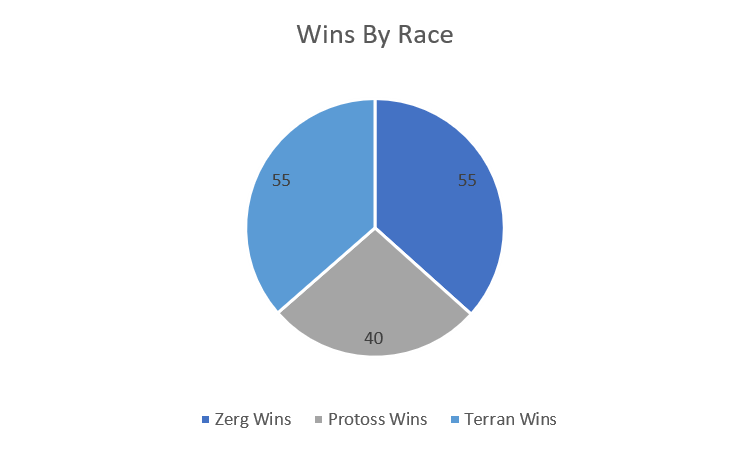
\includegraphics[width=0.5\textwidth]{RacePie}
		\caption{A pie chart representing the average win rate \% for the three races, based on the results obtained from table 1.}
		\label{Fig4}
	\end{figure}
	\subsection{Metrics}
	
	Initially, the StarCraft Bot was to be measured on its success in these two metrics:
	\begin{itemize}
		\item \textbf{Time Survived} (Average of 13 minutes or above)
		\item \textbf{Endgame Condition} (Whether the Bot wins the game or looses)
	\end{itemize}
	These metrics were obtained from the results from the AIIDE 2017 StarCraft Competition, which found that the average time of each game was 13-minutes, and the quickest average being 8-minutes and the longest being 19-minutes. The win ratio of the Bots vary substantially from 17.21\% to a high 83.11\% as can be seen in Table 2 \cite{Results}. 
	
	After presenting these findings, it was discussed that the metrics required a greater level of merit, to achieve this, the metrics were modified using the preliminary results and further inspection of the Bots within the literature. As can be seen in fig 6, the mean win rate for the Bot was 50\% and within the literature, the win rate ranged from 54-91\% \cite{ELGoal,Swen,OnlineEvo,GoalDriven}. The literature Bots were faced against both competition Bots and in-built Bots which came with StarCraft.
	
	From the preliminary results obtained from table 1, the mean game time was 14:20, with the longest mean being 19:24 and the shortest mean 6:05. No papers that were reviewed for this research focused on average game length, they seemed only concerned with win\% or Bot efficiency in a focused area of functionality. For the purposes of this paper, game length will be measured and analysed to measure countering the rush tactic. As defined on the Liquipidiea website "Mid-game is the period in a match where the strategy of the early game can come together" and "Mid-game typically starts between 7 and 12 minutes" \cite{Liqui}. This supports the metric that if the Bot survives past the 10-minute mark then it will have successfully countered the rush tactic. 
	\newline
	
	For the final metrics that the Bot will be measured on will be as follows:
	\begin{itemize}
		\item \textbf{Average Game Length} (Average of 14 minutes or below)
		\item \textbf{Average Win Rate} (Win Rate above 50\%)
	\end{itemize}
	
	Through these revised metrics, the effectiveness of the Bot will be determined, if the Bot obtains an average game length of 14 minutes or less, and or has a win rate of 50\% or higher it will support the statement that it is effective. Though if the Bot fails at achieving these goals it will support the NULL hypothesis.
	
	\subsection{Testing}
	The Bot was faced against the open source competition Bots, 400 matchups were simulated, 80 of which the Bot presented in this paper took part in. The environment chosen to test the Bots was the same as the competitions run by D. Churchill, this method of testing was chosen as it provided a ready-made, well-validated method for testing the Bot.
	
	During testing, there was a total of 10 Bots including the Bot that was developed for this research, for the rest of this paper will be referred to as POSH-bot. To choose these Bots, three were selected from the top of the board, three from the middle and three from the bottom. They will be selected from the AIIDE 2016 competition, to keep the experiment as fair as possible each Bot in each tier will consist of each of the races, where that is not possible, a substitute has been made \cite{2016}. AIIDE 2016 was chosen as all the Bots required for testing were available for download. The final Bots that POSH-bot will be facing consist of 4 Terran, 3 Protoss and 2 Zerg, a Zerg was substituted for a Terran as the original Zerg Bot chosen continued to crash throughout the preliminary testing. It was also judged that it would not make a significant difference to the results as one of the Zerg Bots has such a high win rate.
	
	The 10 Bots will be playing on 3 1v1 maps, traditionally there is a selection of 2v2 maps as well. For the purposes of this research, only the 1v1 maps were used as it was judged that on larger maps POSH-bot would have timed out more often, thus resulting in more skewed results. The Bots played for 9 rounds to total 400 matchups with one winner and one looser, the score and game length was also recorded. The three maps used were,(2)Benzene, (2)Destination, (2)HeartbreakRidge, all are available from the D. Churchill's GitHub page for the tournament manager \cite{Tournament}. 
	
	To set up the testing environment a VM was required to run several instances of StarCraft, and the STM. Once the virtual machine was installed a 64-bit operating system had to be installed on the VM, a 64-bit version was required as the STM needed a minimum of 2 Central Processing Unit (CPU) cores to run alongside Starcraft. Then once the VM is set up correctly, the server was launched alongside two clients, one on the host machine and one on the VM. Once the three programs have been launched the user chooses how many rounds the tournament should last, and the rest of the process is automated, the STM will select the correct Bots, send them to the clients and launch the game. After each game the process would begin anew until the tournament was complete, this process took approximately 16 hours. 
	\begin{table*}[]
		\centering
		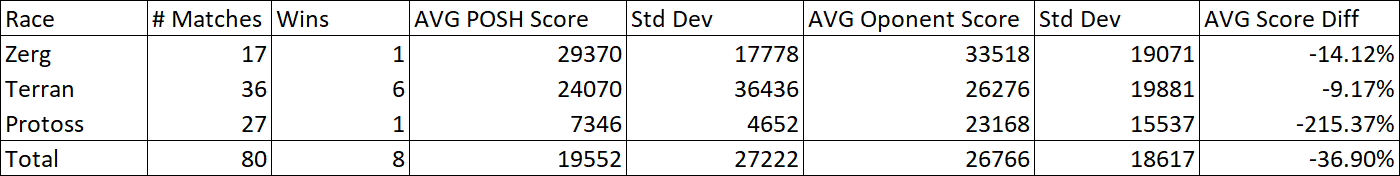
\includegraphics[width=\textwidth]{POSH-botWin}
		\caption{Results from the 80 matches that the POSH-bot described in this paper took part in against the competition Bots on three 1v1 competition maps.}
		\label{Table3}
		\centering
		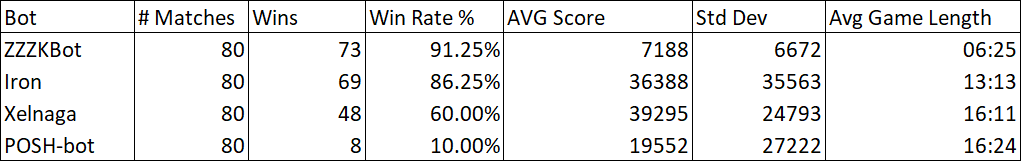
\includegraphics[width=\textwidth]{TopThreeWin}
		\caption{Results from the top three Bots of each race, ZZZKBot(Zerg), Iron(Terran), Xelnaga(Protoss), compared to POSH-bot}
		\label{Table4}
		\centering
		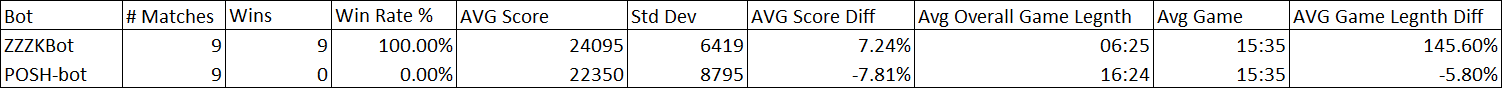
\includegraphics[width=\textwidth]{PvsZ}
		\caption{Closer inspection of the results comparing matches between ZZZKBot and POSH-bot}
		\label{Table5}
	\end{table*}
	
	\section{Results \& Analysis}
	After the implementation of the three chosen strategies, and final testing stages within the tournament manager, the results contained in table 7 located in the appendix came forth. From this other tables were produced, 1 and 5 were produced automatically by the STM, table 2, 3 and 4 were manually created. Though
	
	Investigating POSH-bot facing each race individually, from the results in table 2, under the average game length, the shortest games were against the Protoss with the average game lasting 11:48s and a 3.7\% win rate. POSH-bot also proved less efficient in scores with a -215.37\% difference. This shows that the strategy used by POSH-bot was flawed, as the average game time was 11:48s this indicates that it was the early-mid game, meaning that the early game strategy for the enemy was coming into fruition and POSH-bot failed to counter it. This resulted in the low 3.7\% win rate and substantial difference in score. Though the games ended earlier, the average game length was above 10 minutes, which would indicate that any early rush attempts made by the opponent were countered.
	
	When faced against the Zerg POSH-bot had a similar win rate as to when it faced the Protoss of 5.88\%, but did considerably better with its scores, with a lesser difference -14.12\%, however, the game length on average lasted for 16:46s. Though POSH-bot still failed to achieve a high win rate against the Zerg it did, however, make the matches last longer, past the 15-minute mark. This indicates that the Zerg rush was completely countered, as at this point any early game strategy would have finished and that game was well into mid game. Which also suggests that the strategy employed against the Zerg was successful up until mid game. Another indication of POSH-bot fairing better against the Zerg is the score difference.
	
	The win rate when against Terran was a higher 16.67\%, all 6 of these victories were against the same Bot which had a win rate of 18.52\%. The score difference was lower with -9.17\% and the longest average game length of 19:41s. This suggests that the strategy employed to counter the Terran faired better than the others, likely due to the game lasting past the 15-minute mark allowing the strategy to be fulfilled. The score also supports this as there is a smaller difference means that the POSH-bot managed to counter any rush attempt and produce units to fight.
	
	When inspecting the differences between POSH-bot and the three top Bots for each race in table 3, POSH-bots average game length was close to the same as its counterpart Xelnaga with both having 16:24s and 16:11s respectively. This indicated that POSH-bots strategy succeeded in countering any early rush attempt. Their win rates were considerably different, with POSH-bot having 10\% and Xelnaga claiming 60\%, and coming fourth overall in the testing. Iron a Terran race has a win rate of 86.25\% and an average game length of 13:13s, both of wish were better than the results POSH-bot obtained. ZZZKBot who came out on top during testing managed to secure a 91.25\% win rate, and an average game length of 6:25s. This would indicate that Iron and ZZZKbot's ability to successfully complete an 
	
	Upon closer inspection in table 4, the results obtained from the matches between ZZZKBot and POSH-bot. Though ZZZKBot had a win rate of 100\% the average game length when matched against POSH-bot increased by 146.6\%, both Bots scores were close with a 7\% difference. Though with Iron the game length was decreased by 37.7\% and by 11.98\% by Xelnaga suggesting that POSH-bots early game rush counter was successful against any Zerg attempt, but was hard countered by a Terran vulture and factory rush. Xelnaga also being stronger earlier that POSH-bot attributed to the faster games. Though performing a left-handed t-test on all the results for game length for all matches involving POSH-bot the following results were obtained:
	
	\begin{figure}[H]
		\centering
		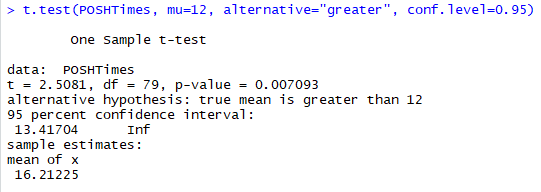
\includegraphics[width=0.5\textwidth]{RPoshTimeLeft}
		\caption{A left sided t-test performed within R Studio for all game lengths on all matches involving POSH-bot.}
		\label{Fig5}
		\centering
		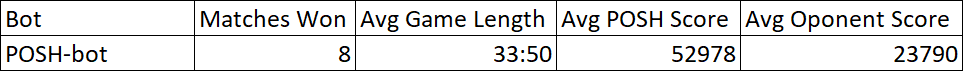
\includegraphics[width=0.5\textwidth]{PoshWinsandScore}
		\caption{An overview of POSH-bots victories over its opponents.}
		\label{poshonly}
	\end{figure}
	
	From this figure a the p-value is near zero which indicates that the null hypothesis can be rejected, in this case, it was to filter out the matches against Iron, by setting the $\mu$ to 10 for the time that a game transits into mid game and in general a rush can no longer be considered a rush. 
	
	During the matches where POSH-bot won as shown in figure 7, on average the games lasted 33:50s, with an average score much higher than that of the opponent. These were most likely timeouts, where the game exceed their maximum frame count quota as stated within the STM readme file \cite{Tournament}. Though victory is awarded to the Bot with the highest score.
		
	After some investigation it was discovered that there may be a correlation between game length and and win rate as shown in figures 8 and 9. Figure 9 shows that there may be a negative correlation between these two values.
	\begin{figure}[H]
		\centering
		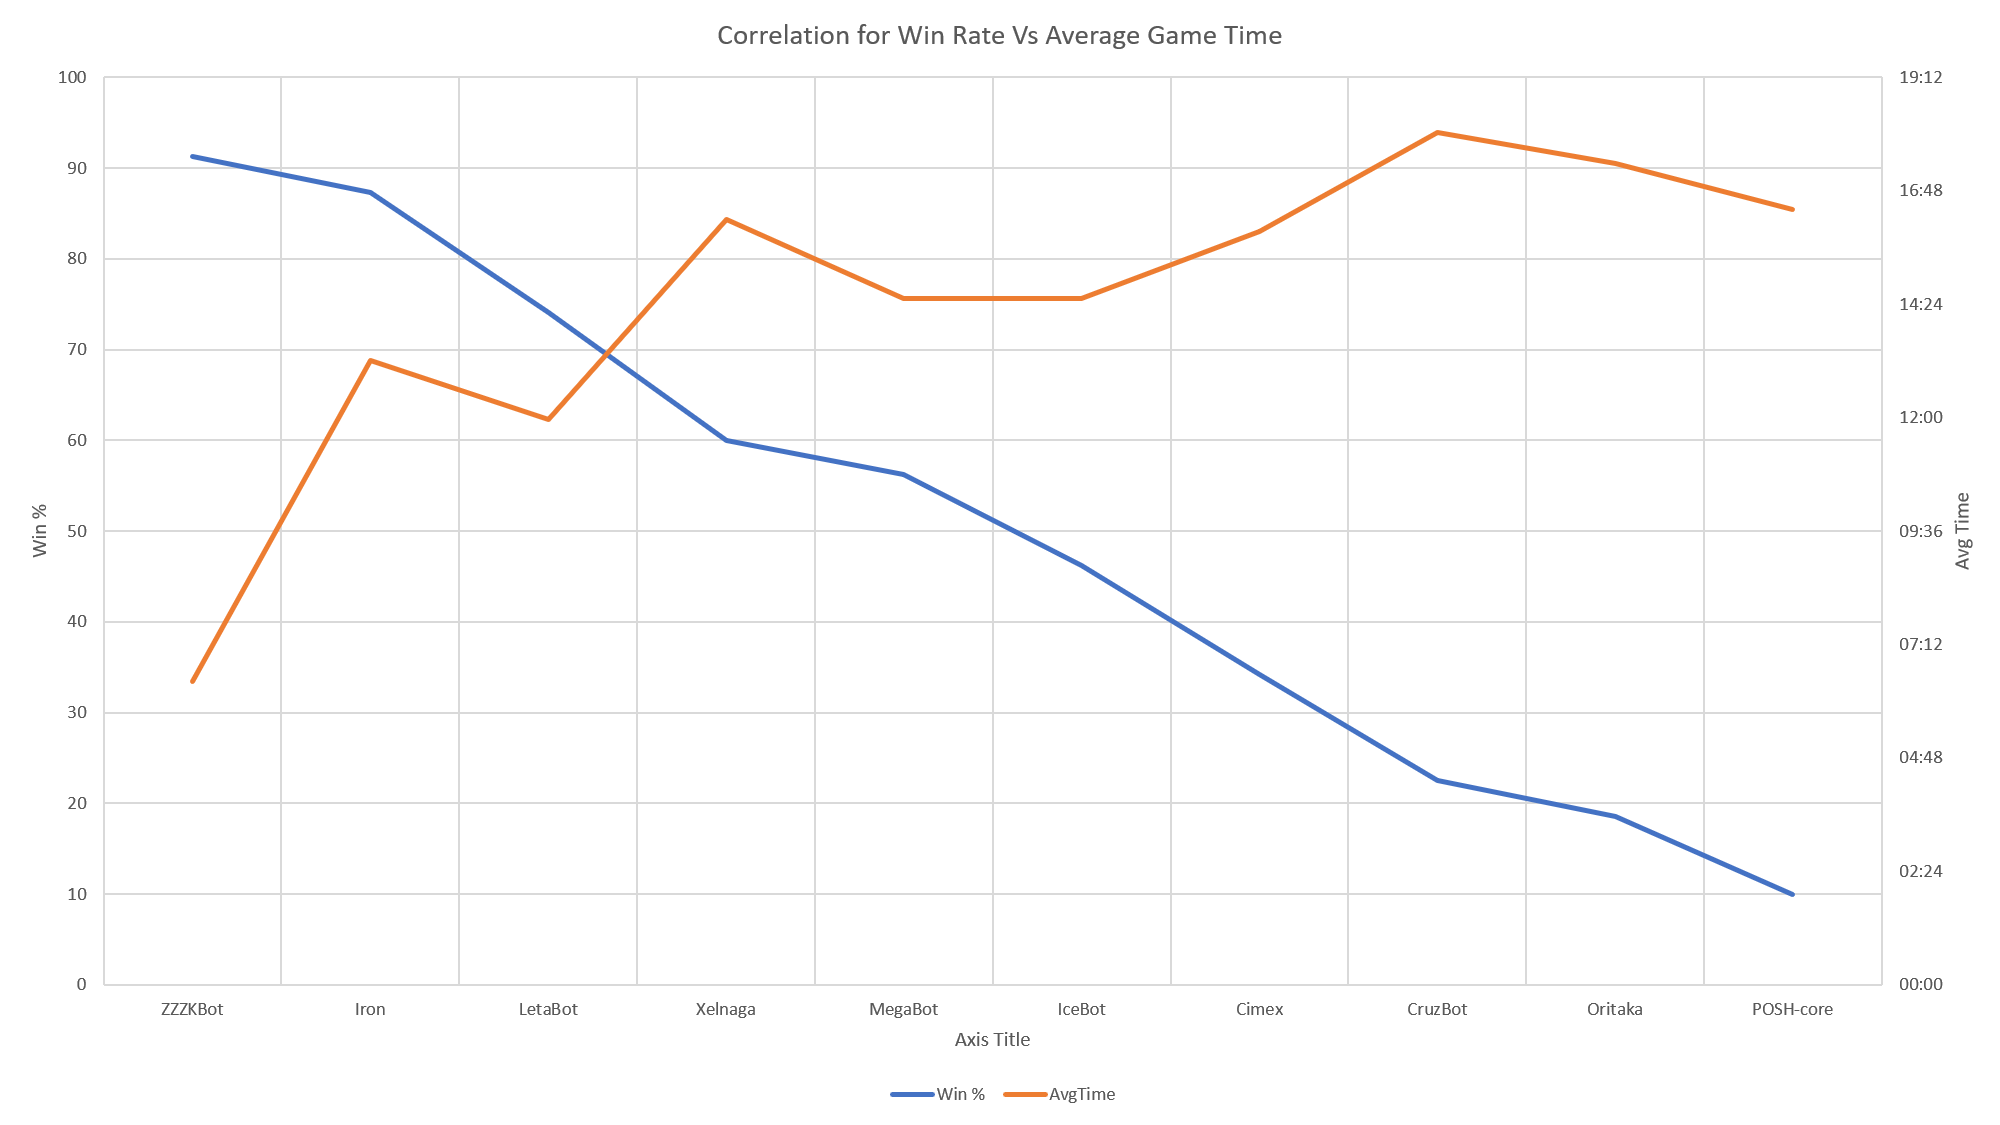
\includegraphics[width=0.5\textwidth]{WinTimeLineWithBot}
		\caption{A line graph showing both the win rate and game length for all the Bots, starting with the highest win rate on the left, based on the results obtained from table 1.}
		\label{Fig7}
	\end{figure}
	\begin{figure}[H]
		\centering
		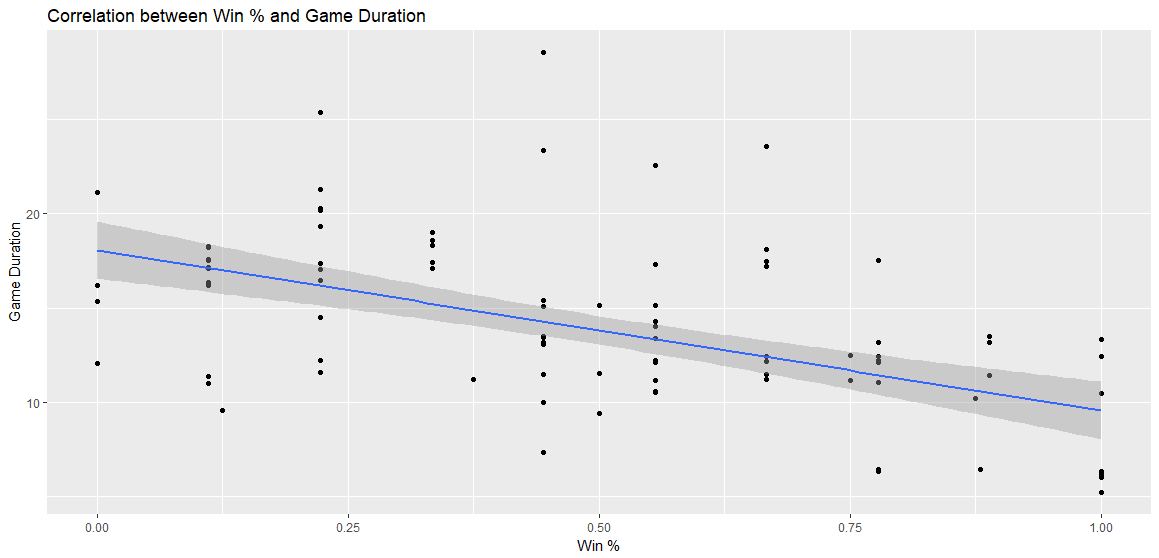
\includegraphics[width=0.5\textwidth]{ScatterWinvsDurLine}
		\caption{A scatter plot showing a negative correlation between the win rate and game length, based on the results obtained from the preliminary experiment. Each dot represents an average win rate and average game length for each bot during each round.}
		\label{Fig8}
	\end{figure}
	\section{Discussion}
	It is clear from these results that the Bot was not by the metrics defined in this paper, effective in its use of the implemented strategies, thus confirming the null hypothesis of hypothesis 3 that the Bot cannot achieve above a 50\% win ratio in its current state. This was not entirely unexpected as during early testing there was evidence that the strategies provided from Liquipidia were not going to be very effective, as they relied on the Bot scouting and building immediately as the game started. As the system could not compute its actions instantaneously the Bot could not execute the strategies in time before the enemy Bot had built a larger force. The framework is too slow and needs altering, and as this was not the focus of this research would have been an improper use of resources.
	
	Though the Bot did achieve a win rate greater than 0\% and therefore supporting hypothesis 2. Upon further inspection of the replays of the games that POSH-bot won against Oritaka a Terran Bot, it became clear the victories accounted for the ability to counter a Terran Marine rush. Due to its similarity to the Zerg rush (sending in weak cheap units) it was easily countered by POSH-bot and it became apparent that this was the main focus Oritaka and once POSH-bot acquired some DT's it easily overpowered Oritaka and destroyed its main base. Though most of the games ended in a timeout, victory was awarded to POSH-bot due to the substantial score difference.
	
	As evidenced by the consistent increase in times for the ZZZKbot's games and POSH-bots ability to survive past the 10-minute mark, as well as the t-test, hypothesis 4 can be supported. 
	
	As shown in figure 7 the average game length for POSH-bots winning matches is much greater than 14 minutes, thus rejecting hypothesis 1 and supporting the null. This was likely due to the lack of scouting abilities within POSH-bot, along with a present bug in the software where the units would not attack correctly, causing the units to not move after reaching the centre of the enemies base. 
	
	\subsection{Analysis of final Software}
	Though two of the hypothesis can be supported, the rearranging two were rejected, this is due to issues that could be improved on in the software. This section will identify those issue and present potential fixes for future work.
	\newline
	
	\subsubsection{Framework}	
	Though once the system was complete and all the behaviours needed were present and creating plans ware a relatively quick process, it has one major disadvantage. The Bot can only execute one action at a time, for example, when the executes the "ProbeScoutToEnemyBase" action it must wait for the entire action to be executed before moving on to the next. This has a negative effect on the design of the Bot as it must be created in such a way that it can be effective while being limited to only one action at a time. A potential work around for this would be to use parallel plans, this would involve having multiple plans working in unison one separate actions to drive the Bot.	
	
	Another issue presented by this software is that it is CPU intensive and at times can slow down the game simulations considerably, this makes testing time increase, there is not much that can be done about it, as the c\# is being translated into c++ for the BWAPI to translate into StarCraft commands. Though ensuring that while loops and for each loops are kept small and only used when absolutely necessary would help to alleviate this issue.
	
	When compiling the bot everything must be run in administrator mode, a minor inconvenience when developing the bot as the bot would launch in this mode when Visual Studios was run with administrator privileges. The software required this as without these privileges the Bot was unable to communicate with BWAPI ad function. The major inconvenience of this requirement came when attempting to launch the Bot using a custom batch file, as the batch file had to launch in admin mode, to achieve this the windows user setting had to have security disabled, so admin privileges were given automatically and the operating system would not request permission. If this was not done then the tournament manager would be unable to launch the Bot and all testing involving the Bot would have to be done manually.
	
	The results for the mirror matches were not unexpected as during development these matches proved the most difficult to implement a strategy for, as both factions can create units at the same rate. As the framework had issues communicating with the game this slowed down the speed of the bot, giving an advantage to any other Protoss the Bot faced. 
	\newline
	\subsubsection{Tournament Manager and Virtual Machine}
	When using the STM an issue that arrose was that only one instance of StarCraft could be run at a time, which required the use of a VM. The issue with this was that if the VM was not set up exactly as needed, the client would not connect to the server/other client, which caused the whole system to not work. This was mainly an issue with the operating system and networking set-up in the VM, but the issue could have been avoided by allowing the STM to launch multiple instances of StarCraft on one machine. StarCraft and the client only require one CPU core each to run plus another for the server, most modern computers hour an octicore CPU, which would allow for 5 core to be used by the clients and StarCraft. 
	
	The STM when running can only allow clients with different IP's to join each other in game, otherwise the game will not recognise that there is a game to join. If the VM was not set up correctly it would share the same IP address as the host machine, which to a user who is unfamiliar with VM software could prevent the use of the STM entirely. A fix that enabled the software to work in this instance was to reinstall the VM with admin privileges which seems to install extra networking adaptor options allowing for the use of a separate IP adress to the host machine, which in turn allows the clients to connect.
	
	When running the STM all firewalls have to be turned off and the registry altered to allow seamless networking between the clients and server, this posses a very high security risk to the users system and could potentially be solved if the STM has a local version which runs off a single host machine.
	\newline
	\subsubsection{Plans and Behaviours}
	As the Bot works through the plan it works from top to bottom, working through the drive and stepping into them as needed if the sense is satisfied. Each of these drives can be delayed and skipped to ensure that all drives are triggered, though this should work in theory. In reality if the delay is more than a few micro seconds the change in speed for the behaviours being triggered is noticeable, as the bot must trigger a command several times as BWAPI does not always work. As for if there is no delay put on the drives, the system will crash as it is running faster than the other two systems, POSH and BWAPI, this causes NULL exceptions to be thrown, so there must be a delay present. The designer can however plan the delays in such a way that the plan not only works its was down the drive list but also works back up. This helps with any issues pertaining to the plan getting stuck inside a particular drive, but does not solve the issue, for this it is best to ensure that the senses are set up correctly so the drive is not triggered at all unless it can be resolved. This means that when creating a plan all drives and senses must be precise, as one incorrect number or misplaced drive can break the Bot entirely, so the plan must be checked and tested several times after each change.
	
	Another issue that arrose several times was the placement of buildings, as stated earlier, BWAPI does sometimes not accept a command form the Bot so th command must be sent again. Which caused issues with building placement as the Bot would register that the building was placed though in game it was not, this meant that the placement and build functions had to be triggered multiple times. 
	
	The Bot currently uses a Fibonacci spiral to locate a suitable build location which should always return a viable option, which is why the Bot currently builds its structures in the immediate vicinity of the main base. This needs to be improved upon as the structures currently interfere with resource gathering, a simple solution would be to implement another strategy that takes advantage of the choke points, this would move the build location to another area. Also as the POSH-bot is Protoss the buildings can only be placed near a Pylon, so another option is to change the build location to each Pylon, though this can cause issues if a Pylon is destroyed, so a list of Pylons would have to be maintained. This solution would force the Bot to build around any Pylon so the only structure that would need changing in its placement would be the Pylon, rather than changing the entire placement system.
	
	Currently there is a large delay between when the game begins and when the Bot can trigger certain actions, for instance, scouting, a pivotal part of an opening strategy. This delays the Bot from being able to perform certain functions like building at its natural early on or harassing the enemy immediately as the game begins. This has cased issues when designing the plan, as th strategies required immediate scouting but the final design had to work around that by triggering the scouting later in the strategy.	
	\begin{table*}
		\centering
		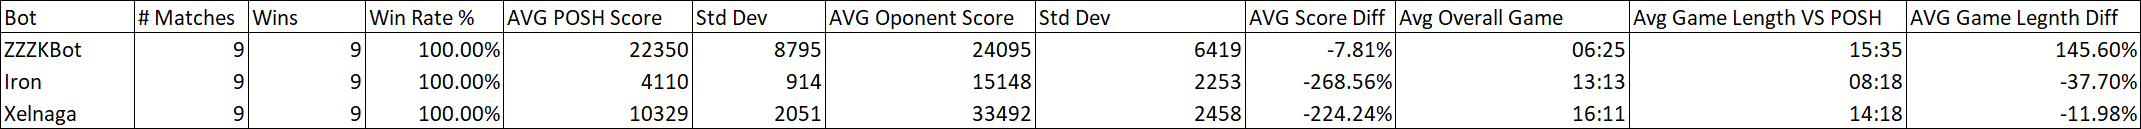
\includegraphics[width=\textwidth]{PvsBots}
		\caption{A line graph showing both the win rate and game length for all the Bots, starting with the highest win rate on the left, based on the results obtained from table 1.}
		\label{Table6}
	\end{table*}
	
	\section{Future Work}
	Though the null hypothesis was confirmed, this work provided an interesting find, that there is a possible correlation between the win rate and game length. A proposed question for future work would be if there is a correlation between them. This would be an interesting find as it could be used to alter the design of Bots to facilitate fast strategies, and through the Zerg implemented a rush tactic which is inherently fast, it would be interesting to see how and Bot using Terran or Protoss would cope with similar strategies.
	Altering the artefact to have executable time set as a priority during development would be an advantage for this as the current software can not keep up with the other Bots in its current state.
	
	An alternative option to solve this issue is to create another plan to run in parallel to the original. This will allow the Bot to execute multiple behaviours at the same time, rather than executing one and having to wait for it to finish before moving on to the next. This would, for example, allow the Bot to build up their base, scout and manage their army at the same time. This would involve precision planning as each plan would have to ensure they do not execute the same action at any point. This was not the primary focus of the artefact, as the framework would have to be modified to allow the use of parallel plans.
	
	Using parallel plans would provide an interesting premiss for designing a Bot. The Bot could have multiple plans, each focusing on a separate component of the game, these could be combat, base building, resource management or defence. Creating a Bot with this capability would provide a challenge in its design as the plans would have to communicate with each other to allow the correct execution times, and it would have to ensure there are no conflicts of interest when managing units. This could be solved with an order of priority or a threat calculation, so the defence can take over from the combat plan if the Bot is losing its base.
	
	A potential improvement to this work could be to investigate the scores of the Bot as in many cases the POSH-bot may not have won but may have performed well as reflected by its scores. As this was not the focus for effectiveness in this paper it could provide a more granular method of evaluating its performance. 
	
	A further step that could be taken is to allow the Bot to construct its own plans with neural networking. It would allow the Bot to learn from pre-built strategies and alter them accordingly as it played a number of matches.
	
	\section{Conclusion}
	In games there are many way to create AI and many game to create AI in, for this work StarCraft was chosen a a platform in which to create one such AI. Creating an effective AI or Bot, for StarCraft can be a challenging task, to which much research has been done, this paper reviewed the literature in this area to analyse the methods used for such a task. After this analysis several questions and hypothesis were presented and a method was created appropriate to solving these questions and supporting the hypothesis.	In this work a bot for StarCraft was presented which used expert strategies sourced from the community surrounding the game, that was tested against several other bots which have participated in the annual AIIDE StarCraft AI competition. The tools that were used were presented as well as the life cycle involved with the Bots creation, once complete the Bot was then tested in a competition environment against Bots that were entered into the 2016 AIIDE StarCraft AI competition. The results were then recorded presented and analysed, after which a discussion was held on the implications of the results, followed with an analysis of the final software used and potential future works. 
	Though the Bot did not fair as well as was hoped, it did prove an interesting challenge, as the design of the Bot was the greatest challenge, as the limitations of the frameworks speed and the way the plans operated had to be circumvented to produce a viable artefact. In this case the Bot presented was not effective in its use of expert strategies, that being said, the Bot did achieve a greater than 0\% win rate, plus the initial rushes were countered, supporting two of the hypothesis presented, showing potential for improvement. For any future work it would be recommended that strategies are kept as simple as possible while maintaining and effective strategy or employ the use of parallel plans to make the Bot more efficient in carrying out that strategy.	
	
	\section{Acknowledgements}
	I would like to thank Swen Gaudl for his help in the creation of this dissertation, without his guidance and patience this work would not have been produced.
	
	I would also like to thank my peers within the BSc for their continuous support throughout this course.
	
	Also, a thank you to Dr.Ed Powley and Dr.Michael Scott for their unyielding dedication to this course ensuring that it continues to be developed to provide the highest quality education.
	% references section
	
	\bibliographystyle{IEEEtran}
	\bibliography{references}
	
	\section{Reflective Addendum}
	If there is one this I have learnt through writing this paper and creating the Bot is that it requires patience and determination. When I began this journey I knew nothing about POSH plans, StarCraft Bots, BWAPI or even any C\#, after taking this project on I realised that it was a bigger deal that I first anticipated, but 
	
	% Appendices
	\appendix
	\begin{table*}[]
		\centering
		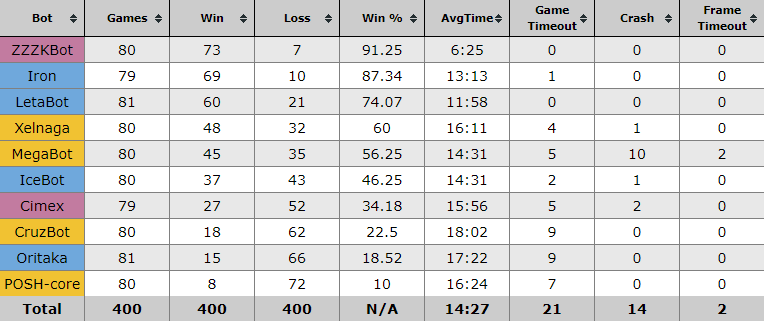
\includegraphics[width=\textwidth]{STMResultsWithBot}
		\caption{The HTML results table produced by the StarCraft Tournament Manager \cite{Tournament}. Blue represents Terran, Purple represents Zerg, and Yellow represents Protoss}
		\label{Table2}
	\end{table*}
	\begin{table*}
		\centering
		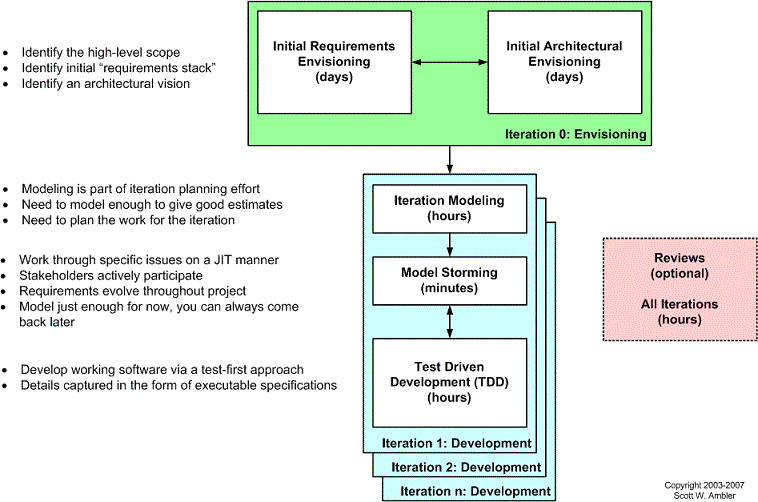
\includegraphics[width=0.75\textwidth]{AMDD}
		\centering\caption{The Agile Model Driven Development (AMDD) lifecycle \cite{AMDD}}
		\label{Fig10}
		\centering
		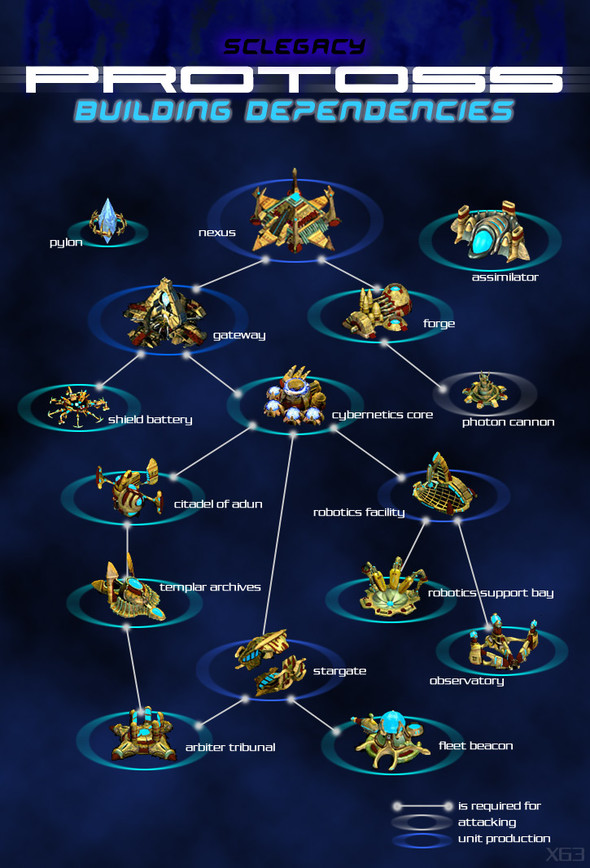
\includegraphics[width= 0.5 \textwidth]{ProtossTechTree}
		\centering\caption{The Tech tree for Protoss, to be able to produce Datk Templar's from the Gateway, Protoss must fist have the Templar Archives. To produce Dragoons the Cybernetics Core must be present, Zealots can be trained as soon as the Gateway is built \cite{Tech}}
		\label{Fig11}
	\end{table*}
	\begin{table*}
		\centering
		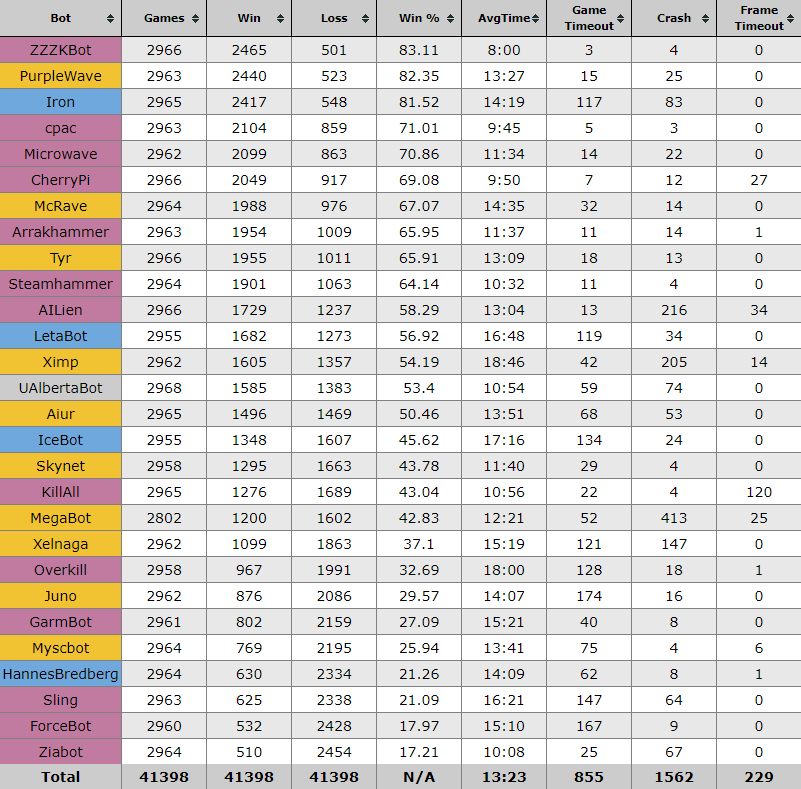
\includegraphics[width=\textwidth]{2017}
		\caption{Results of the 2017 AIIDE StarCraft AI Competition Sourced from the official website \cite{Results}}
		\label{table2}
	\end{table*}
	\begin{table*}
		\centering
		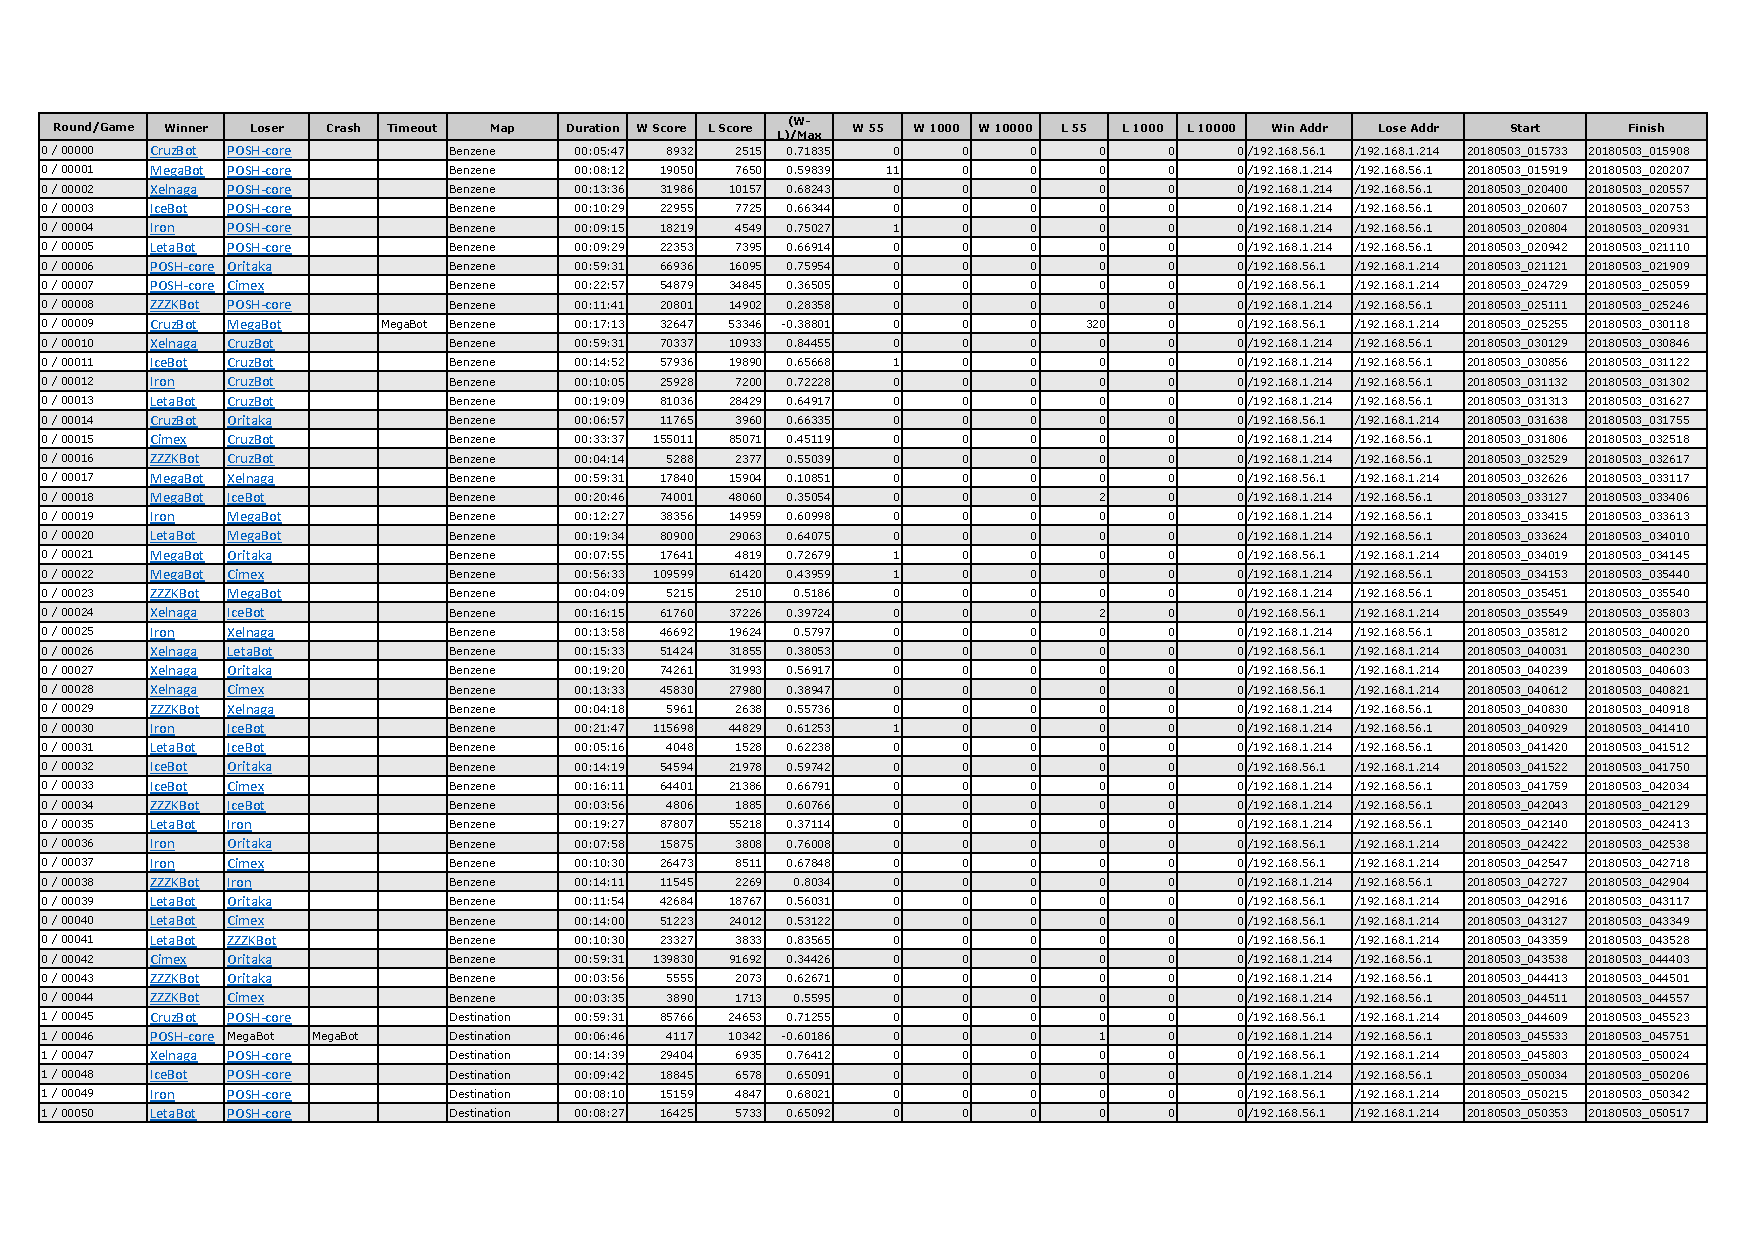
\includegraphics[width=\textwidth]{BotResultsFullTable}
		\caption{An exert from the full table of results produced by the STM}
		\label{table3}
	\end{table*}
	%\listoftodos[Notes]
	
	% that's all folks
\end{document}
